% =====================================================================
%  Datasets_Report.tex -- SIMPLE team guide to the datasets.
%  (The detailed version is Datasets_Report_Detailed.tex/pdf.)
%  Build: tectonic Datasets_Report.tex
% =====================================================================
\documentclass[11pt,a4paper]{article}
% =====================================================================
%  report_preamble.tex -- shared preamble for the stand-alone
%  Datasets and Algorithms reports (article class, A4).
% =====================================================================
\usepackage[T1]{fontenc}
\usepackage[utf8]{inputenc}
\usepackage{mathptmx}
\usepackage[a4paper,margin=2cm]{geometry}
\usepackage{amsmath,amssymb}
\usepackage{graphicx,xcolor}
\usepackage{tikz,pgfplots}
\pgfplotsset{compat=1.18}
\usetikzlibrary{positioning,arrows.meta,calc}
\usepackage{booktabs,array,multirow,tabularx,longtable}
\usepackage{pifont}
\providecommand{\checkmark}{\ding{51}}
\usepackage{enumitem}
\setlist{itemsep=1pt,topsep=3pt,parsep=0pt}
\usepackage[font=small,labelfont=bf]{caption}
\usepackage{float}
\usepackage{cite}
\usepackage{url}
\usepackage[colorlinks=true,linkcolor=hcBlue,citecolor=hcBlue,urlcolor=hcTeal]{hyperref}
\usepackage{titlesec}
\titleformat{\section}{\large\bfseries\color{hcBlue}}{\thesection}{0.6em}{}
\titleformat{\subsection}{\normalsize\bfseries}{\thesubsection}{0.6em}{}
\setlength{\parskip}{3pt}

% ---- Palette (colour-blind friendly) ----------------------------------
\definecolor{hcBlue}{HTML}{2166AC}
\definecolor{hcTeal}{HTML}{1B9E77}
\definecolor{hcOrange}{HTML}{D95F02}
\definecolor{hcPurple}{HTML}{7570B3}
\definecolor{hcRed}{HTML}{B2182B}
\definecolor{hcGray}{HTML}{6E6E6E}
\definecolor{boxBg}{HTML}{EEF3FA}

\pgfplotsset{
  hcaxis/.style={
    tick align=outside, tick pos=left, grid=major,
    major grid style={line width=0.2pt,draw=gray!30},
    axis line style={draw=gray!55},
    label style={font=\footnotesize},
    tick label style={font=\scriptsize},
    legend style={font=\scriptsize,draw=gray!40,fill=white,rounded corners=1pt},
    every node near coord/.append style={font=\tiny},
  }
}

\newcolumntype{L}[1]{>{\raggedright\arraybackslash}p{#1}}
\newcolumntype{Y}{>{\raggedright\arraybackslash}X}

% Highlight box for key take-aways
\newcommand{\keybox}[1]{%
  \par\smallskip\noindent\colorbox{boxBg}{\parbox{\dimexpr\linewidth-2\fboxsep}{\small #1}}\par\smallskip}

\setlength{\parindent}{0pt}

% A simple "dataset card"
% #1 name, #2 one-line what, #3 size, #4 what is inside, #5 our use, #6 link
\newcommand{\dcard}[6]{%
\par\medskip\noindent
\colorbox{boxBg}{\parbox{\dimexpr\linewidth-2\fboxsep}{%
{\large\bfseries\color{hcBlue}#1}\\[2pt]
#2\\[4pt]
\begin{tabularx}{\linewidth}{@{}L{2.6cm} Y@{}}
\textbf{Size} & #3 \\
\textbf{What is inside} & #4 \\
\textbf{How we use it} & #5 \\
\textbf{Link} & \url{#6} \\
\end{tabularx}}}\par}

\title{\color{hcBlue}\bfseries Datasets: Simple Guide for the Team}
\author{Project: Skin Cancer Detection Using Deep Learning}
\date{}

\begin{document}
\maketitle
\vspace{-8mm}

\section*{1. What is a dataset?}
A dataset is a big folder of skin photos where doctors have already
written the correct answer (the \emph{label}) for each photo, for
example ``melanoma'' or ``harmless mole''. Our model learns by looking
at thousands of these labelled photos.

\section*{2. Words you need to know}
\begin{tabularx}{\linewidth}{@{}L{3.6cm} Y@{}}
\toprule
\textbf{Word} & \textbf{Simple meaning} \\
\midrule
Lesion & A spot, mole, or patch on the skin \\
Malignant & Cancer (dangerous) \\
Benign & Not cancer (harmless) \\
Melanoma (MEL) & The most dangerous skin cancer \\
BCC, SCC & The two most common skin cancers \\
Actinic keratosis (AK) & A rough patch that can turn into cancer \\
Dermoscopic image & A close-up photo taken with a special skin magnifier \\
Clinical / smartphone image & A normal photo taken with a camera or phone \\
Mask & A black-and-white image that marks exactly where the lesion is \\
Metadata & Extra patient details: age, sex, body part \\
\bottomrule
\end{tabularx}

\section*{3. The datasets we will use (the plan in one picture)}
\begin{center}
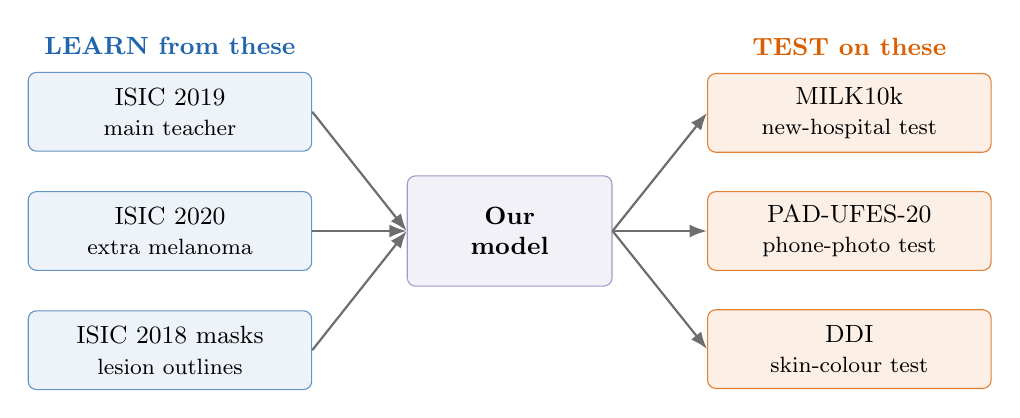
\begin{tikzpicture}[font=\small, node distance=5mm and 10mm,
  tr/.style={draw=hcBlue!70,fill=hcBlue!8,rounded corners=3pt,minimum width=36mm,minimum height=10mm,align=center},
  te/.style={draw=hcOrange!80,fill=hcOrange!10,rounded corners=3pt,minimum width=36mm,minimum height=10mm,align=center},
  md/.style={draw=hcPurple!70,fill=hcPurple!10,rounded corners=3pt,minimum width=26mm,minimum height=14mm,align=center},
  fl/.style={-{Latex[length=2.2mm]},draw=hcGray,thick}]
\node[tr] (a) {ISIC 2019\\\footnotesize main teacher};
\node[tr,below=of a] (b) {ISIC 2020\\\footnotesize extra melanoma};
\node[tr,below=of b] (c) {ISIC 2018 masks\\\footnotesize lesion outlines};
\node[md,right=12mm of b] (m) {\textbf{Our}\\\textbf{model}};
\node[te,right=12mm of m,yshift=15mm] (x) {MILK10k\\\footnotesize new-hospital test};
\node[te,right=12mm of m] (y) {PAD-UFES-20\\\footnotesize phone-photo test};
\node[te,right=12mm of m,yshift=-15mm] (z) {DDI\\\footnotesize skin-colour test};
\draw[fl] (a.east)--(m.west); \draw[fl] (b.east)--(m.west); \draw[fl] (c.east)--(m.west);
\draw[fl] (m.east)--(x.west); \draw[fl] (m.east)--(y.west); \draw[fl] (m.east)--(z.west);
\node[above=1mm of a,font=\small\bfseries,text=hcBlue] {LEARN from these};
\node[above=1mm of x,font=\small\bfseries,text=hcOrange] {TEST on these};
\end{tikzpicture}
\end{center}
\keybox{\textbf{Why two groups?} If we test the model on the same kind of
photos it learned from, it is like giving a student the exact exam
questions they practised. To prove the model really works, we test it
on photos from \emph{other} hospitals, \emph{other} cameras, and
\emph{other} skin colours.}

% =====================================================================
\section*{4. Datasets for LEARNING (training)}

\dcard{ISIC 2019 --- our main dataset}
{The biggest collection of labelled skin-lesion photos with many classes.}
{25{,}331 photos}
{8 classes: melanoma, BCC, SCC, actinic keratosis (these 4 are cancer or pre-cancer), and 4 harmless types. Also age, sex, body part.}
{Main training data. It already contains HAM10000 and BCN20000, so we do \textbf{not} download those again.}
{https://challenge.isic-archive.com/data/}

\dcard{ISIC 2020 (SIIM-ISIC Melanoma)}
{Photos from 2{,}056 real patients, mostly harmless moles.}
{33{,}126 photos (only 584 are melanoma)}
{Melanoma vs.\ not melanoma, plus age, sex, body part, patient ID.}
{Extra melanoma examples and practice with rare cancer, like in real life.}
{https://www.kaggle.com/c/siim-isic-melanoma-classification}

\dcard{ISIC 2018 Task 1 --- lesion masks}
{Photos where experts have drawn the exact outline of each lesion.}
{2{,}594 photos with masks}
{Photo + mask pairs.}
{Train the segmentation model that finds and cuts out the lesion.}
{https://challenge.isic-archive.com/data/}

% =====================================================================
\section*{5. Datasets for TESTING}

\dcard{MILK10k (ISIC 2025) --- new-hospital test}
{The newest ISIC dataset. Each lesion has a normal photo \emph{and} a close-up photo.}
{5{,}240 lesions (10{,}480 photos)}
{11 classes including melanoma, BCC, SCC. Almost all confirmed by lab test (biopsy). Includes skin tone.}
{Final test: does our model work on photos it has never seen? (Remove any photo that is also in ISIC 2019 first.)}
{https://doi.org/10.34970/648456}

\dcard{PAD-UFES-20 --- phone-photo test}
{Photos taken with ordinary smartphones in Brazil.}
{2{,}298 photos}
{6 classes: BCC, SCC, melanoma, and 3 non-cancer types. Includes skin type.}
{Test: does a model trained on close-up photos still work on phone photos?}
{https://doi.org/10.17632/zr7vgbcyr2.1}

\dcard{DDI --- skin-colour fairness test}
{Photos from Stanford with an equal mix of light, medium, and dark skin.}
{656 photos}
{Cancer vs.\ not cancer, all confirmed by biopsy, with skin-tone group.}
{Test: is our model equally good for dark and light skin? (Needs a free sign-up.)}
{https://ddi-dataset.github.io/}

\dcard{PH2 --- small outline test}
{A small, high-quality set from Portugal.}
{200 photos}
{Moles and melanomas, with expert outlines.}
{Test the segmentation model on a different hospital.}
{https://www.fc.up.pt/addi/ph2\%20database.html}

% =====================================================================
\section*{6. Other datasets (good to know, not required)}
\begin{tabularx}{\linewidth}{@{}L{2.7cm} r L{4.6cm} Y@{}}
\toprule
\textbf{Name} & \textbf{Photos} & \textbf{Note} & \textbf{Link} \\
\midrule
HAM10000 & 10{,}015 & Most famous dataset; already inside ISIC 2019 & \href{https://doi.org/10.7910/DVN/DBW86T}{\nolinkurl{doi.org/10.7910/DVN/DBW86T}} \\
BCN20000 & 18{,}946 & Hard cases from Barcelona; already inside ISIC 2019 & \href{https://doi.org/10.6084/m9.figshare.24140028}{\nolinkurl{doi.org/10.6084/m9.figshare.24140028}} \\
SLICE-3D (ISIC 2024) & 401{,}059 & Huge, but only 0.1\% cancer; for future work & \href{https://www.kaggle.com/competitions/isic-2024-challenge}{\nolinkurl{kaggle.com/competitions/isic-2024-challenge}} \\
Fitzpatrick 17k & 16{,}577 & Many skin diseases with skin-colour labels & \href{https://github.com/mattgroh/fitzpatrick17k}{\nolinkurl{github.com/mattgroh/fitzpatrick17k}} \\
Derm7pt & 1{,}011 cases & Doctor's 7-point checklist labels & \href{https://derm.cs.sfu.ca/}{\nolinkurl{derm.cs.sfu.ca}} \\
ISIC Archive & -- & Search and download any ISIC image & \href{https://www.isic-archive.com/}{\nolinkurl{isic-archive.com}} \\
\bottomrule
\end{tabularx}

% =====================================================================
\section*{7. Five simple rules for using the data}
\begin{enumerate}
  \item \textbf{Remove copies.} Some photos appear in more than one
        dataset. Find and delete duplicates before anything else.
  \item \textbf{Keep the same lesion together.} If one mole has 3 photos,
        all 3 must go into training \emph{or} all 3 into testing, never
        split.
  \item \textbf{Never train on the test datasets.} MILK10k, PAD-UFES-20,
        and DDI are only for the final exam.
  \item \textbf{Use the same class names.} Different datasets use
        different names for the same thing (AK, AKIEC, ACK). Make one
        list and convert all labels to it.
  \item \textbf{Cancer photos are rare.} Do not judge the model by
        accuracy alone; check how many cancers it catches.
\end{enumerate}

\keybox{\textbf{Summary:} Learn from ISIC 2019 + ISIC 2020 (+ ISIC 2018
masks). Test on MILK10k, PAD-UFES-20, DDI, and PH2. All are free for
student research. The full detailed version is in
\texttt{Datasets\_Report\_Detailed.pdf}.}

\end{document}
